\section{Overview of \MP{}}

\MP{} aims to identify important factors of memory allocators, which tells programmers not only why , but also the reason of . 

\MP{} is designed as a drop-in library that can be simply linked to applications (and allocators) with the preloading mechanism, which does not require the changing of the code or re-compilation. %Although \MP{} may employ the binary instrumentation to perform a more detailed profiling, such as identifying the instructions within each allocation or deallocation, the binary instrumentation may impose prohibitive performance overhead. With a high overhead, the profiling results may be significantly skewed, such as the waiting time of each lock acquisition inside the allocation. Instead, \MP{} employs the PMU hardware, RDTSC timestamp hardware, and simple counters together to perform the profiling.  
As shown in Figure~\ref{fig:basicidea}, \MP{} intercepts the interfaces between the memory allocator with other components of the system, such as applications, the OS (e.g.,  memory related system calls), and the pthreads library (e.g., synchronizations). At the same time, \MP{} also employs  hardware performance counters to collect more information, such as the instructions, cache misses or TLB misses of each allocation and deallocation, which also does not need to change the code of applications. 
 
\begin{figure}[!ht]
\centering
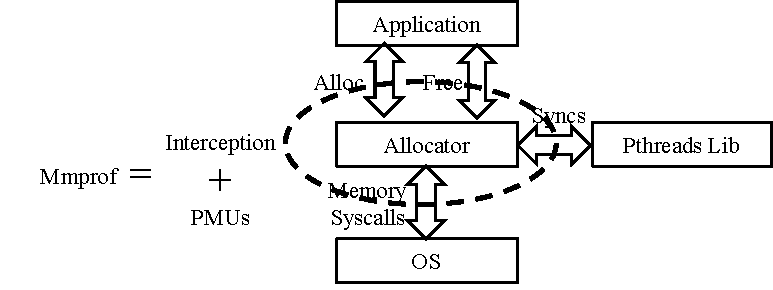
\includegraphics[width=3.3in]{figures/basicidea}
\caption{Basic Idea of mmprof\label{fig:basicidea}}
\end{figure}

Overall, \MP{} focuses on the allocator itself and its potential impact on applications (called as ``application friendliness''). These two factors, when combined together, explain the performance difference of different allocators. \MP{} can assist  allocator developers to identify the potential  design issue, without writing a specialized profiler. It could also help a user to choose an appropriate allocator for specific applications.

In the remainder of this section, we describe the profiled items for each category, and the basic idea of profiling. 

\subsection{Background}

 

\subsection{Basic Idea of mmprof}
\MP{} profiles different types of data as discussed in the following. Among them,  performance overhead, memory overhead, and scalability belong to internal mechanisms of allocators themselves, while the application friendliness focus on the potential performance impact on applications.  
  
\subsubsection{Performance Overhead}

For performance overhead, \MP{} profiles the average data of each allocation and deallocation, instead of the summarized values over the whole execution. Per allocation/deallocation data helps identify internal issues inside, if the data is counterintuitive. For instance, \texttt{DieHarder} is identified to have a very high number (\todo{up to X on average}) of cache misses upon each deallocation, which clearly a deficiency inside. 

First, \MP{} collects the time spending on each allocation and deallocation. It intercepts allocations and deallocations of allocations, and then computes the RDTSC timestamp difference before and after each operation as the execution time. The allocation and deallocation time is a very important metrics on the efficiency of an allocator.  

%TLB read misses/TLB write misses/page faults/cache misses/instructions. They are PMU-based. 
% 

Second, \MP{} further collects hardware PMU events for each allocation and deallocation, where the introduction of PMU is described in Section~\ref{sec:pmu}. The PMU events allow \MP{} discover the specific information of allocations/deallocations without using the instrumentation, such as retired instructions, cache misses, and TLB read/write misses. 

%Based on our understanding, the hardware events, such as retired instructions, cache misses or TLB misses, will help reveal some implementation issues of an allocator. For instance, \MP{} detects that the DieHarder allocator has an excessive number of cache misses and TLB misses upon each deallocation, around 5 times of each deallocation, which is significantly larger than that of other allocators. By examining the code, we found out a serious implementation issue of the DieHarder allocator, which traverses all mini-heaps to identify the placement of each object. Obviously, this implementation is extremely slow, considering that every deallocation has to perform such expensive lookup. By fixing such issues, the DieHarder's performance improves around \todo{20\%}.     


\begin{comment}
Can we integrate the cache misses or page faults for each allocation and deallocation, so that we could identify the issue of DieHarder that invokes many unnecessary cache misses?

If we could correlate cache misses to each thread, then we could do this. 

If allocation and deallocation takes too much time, it could be caused by multiple reasons:

(1) First, it just takes a lot of instructions (could we find out the lapsed instructions for each thread?)
(2) It may be caused by not good algorithm? 
(3) It can be caused by lock contention?
(4) It can be caused by system call related contention?
\end{comment} 

\subsubsection{Memory Overhead}

Based on our understanding, the memory overhead comes from two aspects: the metadata overhead, and the memory inflation. The metadata overhead indicates the physical space used for tracking objects or others. Memory inflation indicates that the actual memory consumption is increased unnecessarily due to some inherent design of a memory allocator. 

Based on our understanding, multiple reasons may contribute to the memory inflation.  Firstly, internal fragmentation, or the alignment overhead, may contribute this. As described before, typically allocators manage heap objects using size classes, in order to enable  memory re-utilization without coalescing or splitting. The difference between the requested size and size class (or mapped pages) is called as alignment overhead or internal fragmentation. Secondly, the memory blowup can contribute this issue as well, where an allocator does not satisfy the request immediately with freed objects. As described in , different per-processor heap will maintain their to reduce the conflict.   

Third, some allocators, especially secure allocators, typically skip some objects. For the memory overhead, \MP{} aims to determine the ratio of each portion, so that it could guide allocator developers to further reduce the memory overhead based on the profiling results. 


It is relatively easy to compute the alignment overhead, as far as the information of size classes is known, which \MP{} utilizes a pre-run program to obtain (as described in Section~\ref{sec:understandingallocators}). \MP{} tracks each memory allocation, and then computes the alignment overhead for each allocation request. \todo{Of course, upon the deallocation, the corresponding alignment overhead will be extracted from the current overhead. But how we could know the actual alignment overhead for each object? It seems that we should store the information of such objects, or we could recompute due to the last object. }

For the memory blowup overhead, \MP{} profiles two types of blowup overhead. One type is simply based on the size of freed objects. If the total size of freed objects is larger than the requested size, but an allocation is satisfied from never-allocated objects, which is consider to be a memory blowup. Another type is based on the total size of freed objects with the same size.  

However, it is extremely challenging to compute  the metadata overhead, since it is difficult to identify the location of the metadata, without knowing (or changing) the detailed design of an allocator. \MP{} proposes a novel way to get the metadata overhead, based on the equation~\ref{eq:memoryoverhead}. That is, the metadata overhead can be computed if the total memory overhead ($Total\_{OH}$), alignment overhead ($Align\_{OH}$), or memory blowup ($Blowup$) is known.   

\begin{equation}
%\vspace{-0.1in}
\label{eq:memoryoverhead}
Total\_{OH}=Metadata\_{OH}+Align\_{OH}+Blowup
\end{equation} 

That is, we could compute the metadata overhead if we could know the total overhead of the heap, given that $Blowup$ and $Align\_{OH}$ can be computed as described above. The total memory overhead is the difference between the total memory consumption of heap objects and the total requested size of heap objects. For the latter one,  \MP{} could increment the size of every allocation, and then decrement the corresponding size of each deallocation.  That is, the question attributes to the determination of the memory consumption of the heap. We noticed that the \texttt{/proc/PID/smaps} file actually contains the size of physical memory for each virtual memory region (in its \texttt{Referenced} field). That is, we could compute the total physical memory consumption by summing up all physical memory of virtual memory regions that are related to the heap. In order to identify all virtual memory regions belonging to the heap, \MP{} intercepts all memory related system calls, and only includes those ones invoked during allocations and deallocations. 

 


%How we could know the total memory consumption? As described in Section~\ref{}, \MP{} intercepts all memory allocations and deallocations. Also,  all memory-related system calls, such as \texttt{mmap}, \texttt{munmap}, \texttt{madvise}, \texttt{mremap}, and \texttt{sbrk}. occurring inside memory allocations and deallocations will be tracked, where the allocator may utilize the  

For memory overhead, programmers only care about the time with the maximum overhead. To achieve this, \MP{} periodically gets the data about the memory overhead, but only shows the data with the maximum overhead to programmers.  
 
\subsubsection{Scalability Analysis} 

\MP{} profiles the scalability issues of allocators as well. Since the contention is the major reason that could significantly affect the scalability of applications, \MP{} focuses on both user-space contention and kernel-space contention. 

\subsubsection{User Space Contention}
For user-space contention, \MP{} obtains the number of lock acquisitions, the average time for each lock acquisition, and the average time spending under the protection of locks. After that, \MP{} could divide the number of the lock acquisitions by the number of allocations, in order to find out whether the allocator substantially acquires the lock or not. Based on our knowledge, some allocators prevents the lock as much as possible, which possibly achieves better scalability. 

The average time for each lock acquisition can be employed to confirm the lock contention inside. \MP{} obtains the average acquisition time for locks without the contention at first. Then it could show whether the lock contention of an allocator is significant high or not.

At the same time, \MP{} also acquires the time within the critical section. This could help expose whether the lock contention is due to the heavy workload inside the critical section or not. This may require the programmers to take two different actions. For instance, if the contention is high, but the average time inside the critical section is low, then this allocator should possibly distribute its management to multiple threads. In contrast, if the average time inside the critical section is high, then the allocator should possibly move some computation out of the critical section. 

%In order to reduce unnecessary contention, \MP{} avoids the cache-line based contention. In particular, it utilizes a thread-local pointer that saves the address of thread-local storage. 

\subsubsection{Kernel Contention}
\MP{} evaluates the kernel contention caused by the allocators, since an allocator may interact with the OS substantially. \MP{} does not require to change the kernel directly to achieve this target. Instead, \MP{} monitors the number and the duration time of memory-related system calls inside the user space, such as \texttt{mmap}, \texttt{munmap}, \texttt{madvise}, \texttt{sbrk}, \texttt{madvise}, or \texttt{mremap}. By examining the source code of the Linux kernel, they will acquire a process-based lock (e.g. \texttt{mmap\_sem}) upon the entry of these system calls, causing the kernel-level contention. If an allocator invokes a much larger number of system calls,  or if the average time spending on a system call is higher than the execution time of this system call without the contention, which indicating significant contention side, then the allocator should be improved. 

\MP{} intercepts the invocations of such system calls, utilizes the RDTSC timestamps to collect the duration time of each system calls, and saves the duration and the number of invocations to the thread-local storage. In the end, it can compute the average time and the number of invocations for each system call. Similarly, the average time can be compared with the time without the contention. Therefore, it is easy to know whether there exists kernel contention or not. Therefore, the allocator can be improved by avoiding such frequent system calls. This method helps to expose some issues of the Glibc allocators, which causes significant slowdown on one application. 

  
%\MP{} also tracks the virtual memory regions by analyzing these system calls. 

\begin{comment}
   the information can be utilized to tell whether an allocator has significant  
As we all know, memory allocators may invoke multiple system calls inside allocation and deallocation. 
User space contention:
How many separate locks are explicitly utilized? 
How many lock acquisitions? How much time are spending on lock waiting for each thread, and in total?

How much time spending on kernel-space contention? For instance, we could infer from memory-related system calls, such as mmap, munmap, madvise, brk, or something else? 

That is, we may have to integrate with SyncPerf for doing this. We will borrow their implementation in order to do this. 
\end{comment}

\subsubsection{Application Friendliness} 
\MP{} further tracks the application friendliness of different allocators, which may explain the performance difference when using different allocators. For application friendliness, \MP{} currently focuses on cache and page level only. For cache, \MP{} focuses on the cache utilization and cache contention rate. For page, \MP{} aims to uncover the page utilization ratio. These factors could substantially affect the performance of applications. 

Cache utilization rate indicates the percentage of cache line are utilized for holding the actual heap data. Memory allocators may significantly affect this ratio. For instance, some allocators (e.g. Linux allocator) may collocate the metadata with the actual heap objects. This method, although improving the speed of memory management, will reduce the cache utilization rate and cause more cache misses unnecessarily. 
Also, if memory allocators cannot quickly re-utilize the freed objects, due to concurrent memory management or using FIFO method to manage freed objects, they can also cause low cache utilization rate. Page utilization rate indicates the percentage of a page that are actively utilized for holding the actual heap data. Similarly, if per page utilization rate is low, it may cause high TLB misses and prohibitive memory consumption. \MP{} detects both cache utilization and page utilization rate, with hardware performance counters support. Basically, \MP{} will sample memory accesses, and check the corresponding cache utilization rate and page utilization rate of the corresponding cache line and page. Overall, \MP{} could report an average cache utilization rate and page utilization rate over all samples. 

\MP{} further checks cache contention rate, which is another important metrics that may significantly affect the performance of applications, although it is not designed as a tool of cache contention detection. For cache contention rate, \MP{} reports the percentage of memory accesses that will cause a cache invalidation.  Similarly, \MP{} also utilizes the sampling mechanism provided by hardware performance counters. Upon each sampled event, \MP{} checks whether the current access causes a cache invalidation or not, and reports the percentage of sampled accesses that could cause the cache invalidation. Basically, \MP{} maintains the cache line ownership for sampled memory accesses, which thread is the last one to write on this cache line. The idea is similar to Cheetah~\cite{Cheetah}. But there are two differences from Cheetah: (1) Cheetah focuses on the identification of false sharing, while \MP{} tries to obtain the basic knowledge about cache contention, including both false sharing and true sharing. During the implementation, Cheetah collects both read/write information of each word, but \MP{} only focuses on the cache line level. (2)  Cheetah only focuses on the cache line with serious issues, which only performs the detection when the number of write accesses on a cache line is over a pre-defined threshold. \MP{} treats every cache line uniformly, and always tracks the cache invalidation information for each cache line. 

\subsection{Technical Challenges}

As described above, \MP{} employs hardware PMUs, RDTSC, and simple counters together to perform the profiling. However, there exists some technical challenges. 

The first and the most important challenge is the \textbf{overhead challenge}, where one careless design may impose up to 100 $\times$ overhead, based on our experience of the development. The huge overhead could be unaffordable even for development phases. More importantly, the significant overhead may also skew the evaluation results unnecessarily.

Other challenges come from the adaption to different allocators. Specific issues include the following ones: (1) How to obtain the specific details of different allocators, such as size class information, type of allocator, metadata size information? (Section~\ref{}) (2) How to design a general but fast lookup mechanism for different allocators (Section~\ref{})? (3) How to profile the user-space contention and kernel-contention for the Glibc's allocator (Section~\ref{}), since it invokes system calls and synchronizations without invoking APIs explicitly?


\subsubsection{Performance Monitoring Units}
\label{sec:pmu}

Hardware Performance Monitor Units (PMU), ubiquitous in modern architectures~\cite{AMDIBS:07, IntelArch:PEBS:Sept09, armpmu}, can be employed to sample memory accesses or hardware-related activities~\cite{DBLP:conf/sc/ItzkowitzWAK03, ibs-sc, ibs-pact, Sheng:2011:RLN:1985793.1985848, LASER, Cheetah}. For hardware-related events, it could collect the number of events, such as the number of retired instructions, page faults, TLB load/store misses. Also, it could sample the detailed information about memory loads and stores, such as IP, timestamps, and memory addresses. Currently, the Linux kernel has supported PMUs starting from 2009 (Linux-2.6.31)~\cite{pmulinuxsupport}, where users could set up performance monitoring via  the \texttt{perf\_event\_open} system call. After collecting events, the user program could fetch these events. 

\subsubsection{Time-Stamp Counter}

\label{sec:rdtsc}

Time-Stamp Counter is a register in all x86 computer that saves the number of cycles since reset. This hardware enables the collection of the time duration accurately with a RDTSC instruction~\cite{coorporation1997using, weaver2013linux}. Comparing to the method of utilizing system calls, such as \texttt{gettimeofday()}, the RDTSC instruction has two advantages. First, the overhead is much lower than issuing a system call, typically around 25-35 cycles~\cite{rdtscoverhead}. Second, it provides a high-resolution timer, with the granularity of cycles, which is much finer than traditional system calls~\cite{pitfallsrdtsc}. For instance, the system call \texttt{gettimeofday} could only provide the microsecond granularity, which is too coarse for measuring the performance of system calls or synchronization overhead.  





